% !TeX spellcheck = en_US
\documentclass[french]{yLectureNote}

\title{Mecanique Analytique}
\subtitle{Physique}
\author{Paulhenry Saux}
\date{\today}
\yLanguage{Français}
%lionels.calmels@cemes.fr
\professor{M.Brut}
\usepackage{graphicx}%----pour mettre des images
\usepackage[utf8]{inputenc}%---encodage
\usepackage{geometry}%---pour modifier les tailles et mettre a4paper
%\usepackage{awesomebox}%---pour les boites d'exercices, de pbq et de croquis ---d\'esactiv\'e pour les TP de PC
\usepackage{tikz}%---pour deiffner + d\'ependance de chemfig
% \usepackage{tabularx}%---pour dimensionner automatiquement les tableaux avec variable X
\usepackage{awesomebox}%---Pour les boites info, danger et autres
\usepackage{menukeys}%---Pour deiffner les touches de Calculatrice
\usepackage{fancyhdr}%---pour les en-t\^ete personnalis\'ees
\usepackage{blindtext}%---pour les liens
\usepackage{hyperref}%---pour les liens (\`a mettre en dernier)
\usepackage{caption}%---pour la francisation de la l\'egende table vers Tableau
\usepackage{pifont}
\usepackage{array}%---pour les tableaux
\usepackage{lipsum}
\usepackage{yFlatTable}
\usepackage{multicol}
\usepackage{tabularx}
\usepackage{booktabs}
\newcommand{\Lim}[1]{\lim\limits_{\substack{#1}}\:}
\renewcommand{\vec}{\overrightarrow}
\newcommand{\N}[0]{\mathbb{N}}
\newcommand{\dd}{\mathrm{d}}
\newcommand{\norm}[1]{||\vec{#1}||}
\newcommand{\fo}{\psi(\vec{r},t)}
\newcommand{\foe}{\psi(\vec{r},t)\*}
\newcommand{\HH}{\hat{H}}
\newcommand{\hb}{\hbar}
\newcommand{\lap}{\nabla^2}
\newcommand{\lapcc}{\frac{\partial^2 }{\partial x^2}+\frac{\partial^2 }{\partial y^2}+\frac{\partial^2 }{\partial z^2}}
\newcommand{\E}{\vec{E}(M)}
\newcommand{\B}{\vec{B}(M)}
\newcommand{\V}{V(M)}
\newcommand{\er}{\vec{e_{\rho}}}
\newcommand{\ep}{\vec{e_{\varphi}}}
\newcommand{\pip}{\pi^+}
\newcommand{\pim}{\pi^-}
\newcommand{\mv}{\mathcal{V}}
\DeclareMathOperator{\Div}{Div}
\newcommand{\rot}{\vec{\mathrm{rot}}}
\newcommand{\grad}{\vec{\mathrm{grad}}}
\newcommand{\qa}{q_{\alpha}}
\newcommand{\qdb}{\dot{q_{\beta}}}
\newcommand{\qb}{q_{\beta}}
\setcounter{chapter}{1}
\begin{document}
\chapter{Calcul variationnel}
\section{Variations et Actions}
Parfois on veut minimiser non pas une fonction mais une fonctionnelle : $$\int L(f'(x), f(x))\dd x$$

\checkInfo{Problème}{Avec une fonction à une variable, pour trouver un maxima, on calcule simplement la dérivée.

Pour une fonction à plusieurs variables, on calcule le gradient.

On s'intersse maintenant aux fonctionelles.
}
\begin{definition}[Fonctionelle]
    Une fonctionelle prend une fonction entrée et donne un nombre réel en sortie
\end{definition}
Par exemple $$\int_x{x_i}^{x_f}L(x,f(x), f'(x))\dd x$$ est une fonctionnelle.

Par exemple, l'énergie potentielle d'un cable entre 2 poteau dont on modélise la corde par $y=f(x)$.

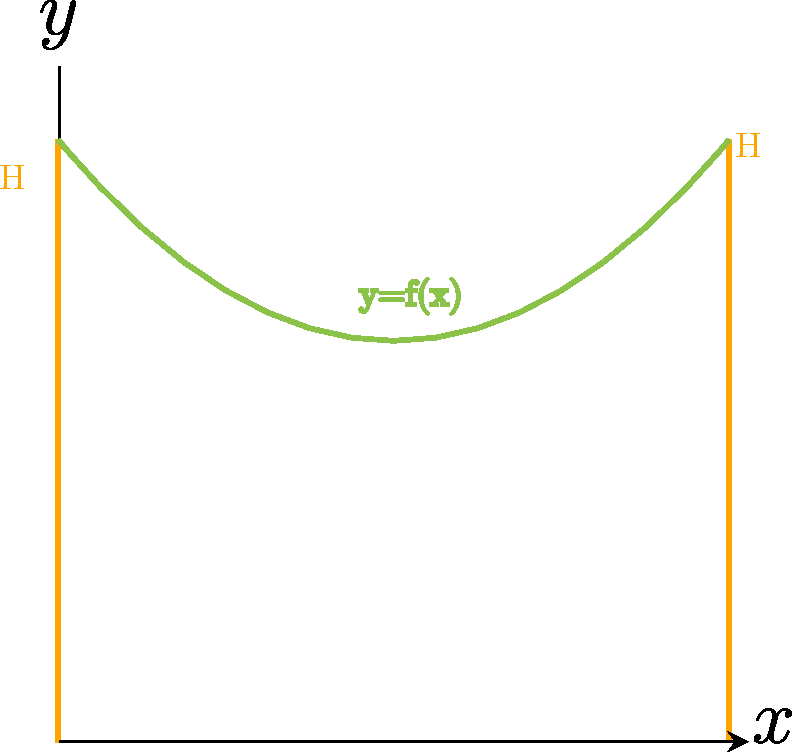
\includegraphics[scale=0.25]{corde.pdf}

%todo c2-1

% Pour minimiser,on va calculer 
% $$\tilde{f}_{f_0(x)+\delta f(x)} \simeq \int_xi^{x_f} \dots \delta f(x)\dd x$$

% On calcule 

% \begin{flalign*}
%     \delta \tilde{f} &= \tilde{f}_{f_0(x)+\delta f(x)}- \tilde{f}_{f_0(x)}\\
%     &= \int_{x_i}^{x_f} L(x, f(x)+\delta f, f'(x)+\delta f'(x))-L(x, f(x), f'(x))\dd x\\
%     &= \int_{x_i}^{x_f} \left(\frac{\partial L}{\partial f'}\delta f'+\frac{\partial L}{\partial f}\delta f+\dots\right) \dd x\\
%     &= \int_{x_i}^{x_f} \left(\frac{\dd }{\dd x}\left(\frac{\partial L}{\partial f'}\delta f\right)-\frac{\dd }{\dd x}\left(\frac{\partial L}{\partial f'}\right)\delta f+\frac{\partial L}{\partial f}\delta f\right) \dd x\\
%     &= \int_{x_i}^{x_f} \frac{\dd }{\dd x}\left(\frac{\partial L}{\partial f'}\delta f\right)\dd x + \int_{x_i}^{x_f} \left(\frac{\partial L}{\partial f}-\frac{\dd }{\dd x}\frac{\partial L}{\partial f'}\right)\delta f \dd x
% \end{flalign*}
% %TODO À corriger
% On retrouve alors l'équation d'Euler-lagrange
% \begin{definition}[Action]
%     Pour q une trajectoire, on a 
%     $$S = \int L(q(t),\dot{q(t)},t)\dd t$$
% \end{definition}


% =========================================================================
% DÉMONSTRATION DE L'ÉQUATION D'EULER-LAGRANGE
% =========================================================================

Pour minimiser ou maximiser une fonctionnelle $\tilde{f}[y]$, on cherche une fonction optimale $f_0(x)$ telle que toute petite variation infinitésimale $\delta f(x)$ autour de $f_0(x)$ (avec $\delta f(x_i) = \delta f(x_f) = 0$ aux bornes) rende la variation de la fonctionnelle nulle au premier ordre : $\delta \tilde{f} = 0$.

On calcule la variation de la fonctionnelle $\tilde{f}$ induite par $\delta f$ :
\begin{align*}
    \delta \tilde{f} &= \tilde{f}[f_0 + \delta f] - \tilde{f}[f_0] \\
    &= \int_{x_i}^{x_f} \left[ L(x, f_0 + \delta f, f_0' + \delta f') - L(x, f_0, f_0') \right] \dd x 
\end{align*}

En effectuant un développement limité au premier ordre (Taylor) de la fonction $L$ au voisinage de $(f_0, f_0')$, on obtient :
\begin{align*}
    \delta \tilde{f} &= \int_{x_i}^{x_f} \left( \frac{\partial L}{\partial f} \delta f + \frac{\partial L}{\partial f'} \delta f' \right) \dd x 
\end{align*}

Pour factoriser par $\delta f$, on utilise la règle de dérivation d'un produit sur le second terme : 
$$\frac{\partial L}{\partial f'} \delta f' = \frac{\partial L}{\partial f'} \frac{\dd (\delta f)}{\dd x} = \frac{\dd}{\dd x} \left( \frac{\partial L}{\partial f'} \delta f \right) - \frac{\dd}{\dd x} \left( \frac{\partial L}{\partial f'} \right) \delta f$$

En réinjectant cette identité (ce qui revient à faire une intégration par parties), la variation s'écrit :
\begin{align*}
    \delta \tilde{f} &= \int_{x_i}^{x_f} \frac{\dd}{\dd x} \left( \frac{\partial L}{\partial f'} \delta f \right) \dd x + \int_{x_i}^{x_f} \left( \frac{\partial L}{\partial f} - \frac{\dd}{\dd x} \left( \frac{\partial L}{\partial f'} \right) \right) \delta f \, \dd x \\
    &= \left[ \frac{\partial L}{\partial f'} \delta f \right]_{x_i}^{x_f} + \int_{x_i}^{x_f} \left( \frac{\partial L}{\partial f} - \frac{\dd}{\dd x} \left( \frac{\partial L}{\partial f'} \right) \right) \delta f \, \dd x
\end{align*}

Comme la variation de la trajectoire est fixée et nulle aux extrémités ($\delta f(x_i) = \delta f(x_f) = 0$), le premier terme s'annule. Pour que $\delta \tilde{f} = 0$ quelle que soit la variation $\delta f(x)$, le théorème fondamental du calcul des variations impose que le terme sous l'intégrale soit nul. 

On retrouve alors l'équation d'Euler-Lagrange :
$$ \frac{\partial L}{\partial f} - \frac{\dd}{\dd x} \left( \frac{\partial L}{\partial f'} \right) = 0 $$

\begin{definition}[Action]
Pour une trajectoire réelle $q(t)$ reliant un point $A$ à un point $B$ entre les instants $t_i$ et $t_f$, on définit l'Action $S$ par la fonctionnelle :
$$ S[q] = \int_{t_i}^{t_f} L(q(t), \dot{q}(t), t) \, \dd t $$
Le principe de moindre action (ou de stationnarité) stipule que la trajectoire physique suivie par le système est celle qui rend $S$ stationnaire ($\delta S = 0$).
\end{definition}

\section{Multiplicateurs de Lagrange et Contraintes}
\subsection{Multiplicateur de Lagrange}
\checkInfo{Rappel : Multiplicateurs de Lagrange}{
Pour trouver les extrema d'une fonction $f(x,y)$ sous une contrainte $g(x,y) = 0$, on utilise la méthode du multiplicateur de Lagrange.
\begin{enumerate}
    \item On introduit une fonction auxiliaire $f_{\lambda}(x, y) = f(x, y) + \lambda g(x, y)$, où $\lambda$ est le multiplicateur de Lagrange.
    \item On cherche les points critiques de $f_{\lambda}$ en résolvant le système :
    \[ \begin{cases}
    \frac{\partial f_{\lambda}}{\partial x} = \frac{\partial f}{\partial x} + \lambda \frac{\partial g}{\partial x} = 0 \\
    \frac{\partial f_{\lambda}}{\partial y} = \frac{\partial f}{\partial y} + \lambda \frac{\partial g}{\partial y} = 0
    \end{cases} \]
    Cela donne les points critiques $(x^*(\lambda), y^*(\lambda))$ qui dépendent de $\lambda$.
    \item On injecte ces points dans l'équation de contrainte $g(x^*(\lambda), y^*(\lambda)) = 0$ pour trouver la ou les valeurs de $\lambda = \lambda^*$.
    \item Les points $(x^*(\lambda^*), y^*(\lambda^*))$ sont les extrema de $f$ sous la contrainte $g=0$.
\end{enumerate}
Cette méthode se généralise à plus de variables et plus de contraintes.
}
On a une fonction de plusieurs variable $F$ On veut déterminer ses extremas sous la contrainte $f(\vec{x})$. Cela se produit en $\vec{x_0}$, alors 
$\vec{\nabla}F // \vec{\nabla}f \Rightarrow \vec{\nabla} = \lambda \vec{\nabla} f$

Si on a 2 contraintes, le sous espace est de dimension $n-2$. Ainsi, $\vec{\nabla}f_1, \vec{\nabla}f_2$ sont $\perp$ à l'espace tangentiel et $\vec{\nabla}F\perp$ à l'espace tengent, donc va \^etre une combinaison linéaire des 2.

\begin{theorem}[Gradient et contrainte dans le cas général]
    $\vec{\nabla}F = \sum_{i=1}^k \lambda_i \vec{\nabla}f_i(\vec{x_0})$
\end{theorem}
\subsection{Application au calcul variationnel}
On veut mnimiser $$S = \int_{t_i}^{t_f}L(q,\dot{q}, t)$$ mais avec la contrainte  intégrale $$\int_{t_i}^{t_f}f(q,\dot{q}, t)\dd t=0$$

On peut écrire
$$\tilde{S} =\int_{t_i}^{t_f} (L-\sum\lambda f) \dd t$$
\subsection{Contrainte locale}
C'est une contrainte que doit satisfaire S à chaque instant. Les multiplicateurs de Lagrange dépendent du temps :
$$\tilde{S} = \int_{t_i}^{t_f}(L-\sum_{i=1}^k \lambda(t)f)\dd t$$

Mais il vaut mieux utiliser les contraintes locales dès le début avec des contraintes scléronomes/hétéronomes.

% =========================================================================
% EXEMPLE : ROULEMENT SANS GLISSEMENT SUR PLAN INCLINÉ
% =========================================================================
\subsection{Exemple : Roulement sans glissement}

On étudie un disque homogène de masse $m$ et de rayon $R$ dévalant un plan incliné d'un angle $\alpha$. Les coordonnées généralisées sont la position du centre de masse $X$ et l'angle de rotation $\theta$.

\begin{center}
    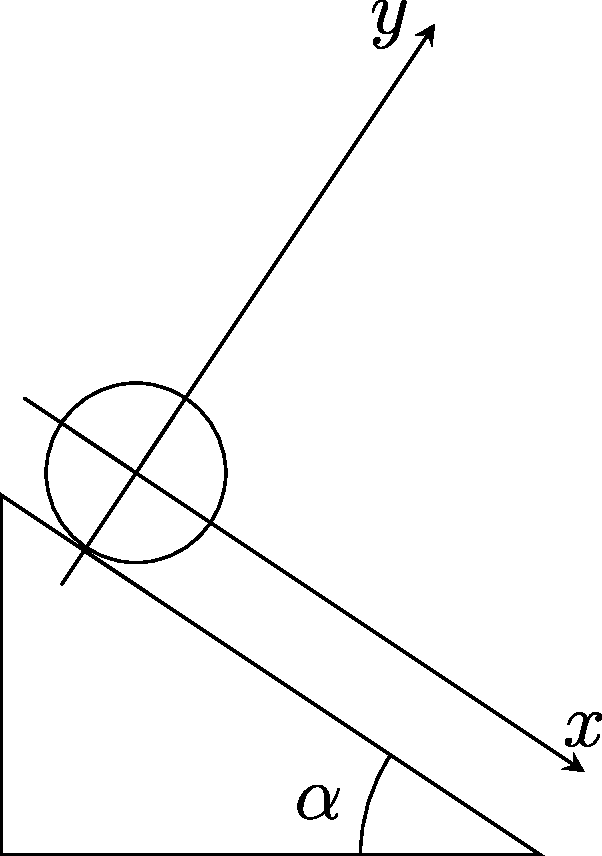
\includegraphics[scale=0.5]{roue.pdf}
\end{center}

\explanation{2}{La contrainte de non-glissement associe cinématique et rotation. On l'intègre au Lagrangien via le multiplicateur $\lambda$ pour trouver la force de réaction.}

\checkInfo{Méthode : Équations d'Euler-Lagrange avec contrainte}{
Quand un système est soumis à une contrainte holonome de la forme $C(q_i) = 0$, on définit le Lagrangien augmenté : $L^* = L - \lambda \, C(q_i)$. 
Les équations du mouvement pour chaque coordonnée $q_i$ deviennent :
$$ \frac{\dd}{\dd t}\left(\frac{\partial L}{\partial \dot{q}_i}\right) - \frac{\partial L}{\partial q_i} + \lambda \frac{\partial C}{\partial q_i} = 0 $$
}

\subsubsection{Énergies et Lagrangien augmenté}
\begin{itemize}
    \item \textbf{Énergie cinétique :} $T = \frac{1}{2}m\dot{X}^{2} + \frac{1}{2}I\dot{\theta}^{2}$ \quad (avec $I = \frac{1}{2}mR^2$ pour un disque homogène).
    \item \textbf{Énergie potentielle :} $V = -mgX\sin(\alpha)$.
    \item \textbf{Contrainte de roulement :} $C(X,\theta) = X - R\theta = 0$.
\end{itemize}

Le Lagrangien augmenté $L^* = T - V - \lambda C$ s'écrit :
$$ L^*(X, \theta, \dot{X}, \dot{\theta}, \lambda) = \frac{1}{2} m\dot{X}^{2} + \frac{1}{2} I\dot{\theta}^{2} + mgX\sin(\alpha) - \lambda(X - R\theta) $$

\subsubsection{Système d'équations du mouvement}
En appliquant les équations d'Euler-Lagrange par rapport à $X$, $\theta$ et $\lambda$, on obtient le système :
\begin{flalign*}
    \frac{\partial L^*}{\partial X} - \frac{\dd}{\dd t}\left(\frac{\partial L^*}{\partial \dot{X}}\right) = 0 &\implies& mg\sin(\alpha) - \lambda - m\ddot{X} = 0  \\
    \frac{\partial L^*}{\partial \theta} - \frac{\dd}{\dd t}\left(\frac{\partial L^*}{\partial \dot{\theta}}\right) = 0 &\implies& \lambda R - I\ddot{\theta} = 0  \\
    \frac{\partial L^*}{\partial \lambda} = 0 &\implies& X - R\theta = 0 \label{eq:lambda}
\end{flalign*}

\subsubsection{Résolution et accélération}
En dérivant deux fois la contrainte, on lie les accélérations : $\ddot{X} = R\ddot{\theta}$. 
L'équation permet d'isoler le multiplicateur de Lagrange $\lambda$ (qui représente ici la force de frottement tangentielle) :
$$ \lambda = \frac{I}{R}\ddot{\theta} = \frac{I}{R^2}\ddot{X} $$

En substituant $\lambda$ dans l'équation dynamique :
$$ m\ddot{X} + \frac{I}{R^2}\ddot{X} = mg\sin(\alpha) \implies \left(m + \frac{I}{R^2}\right)\ddot{X} = mg\sin(\alpha) $$

L'accélération générale du centre de masse vaut donc :
$$ \ddot{X} = \frac{g\sin(\alpha)}{1 + \frac{I}{mR^2}} $$

\tipsInfo{Application numérique selon la géométrie}{
\begin{itemize}
    \item Pour un \textbf{disque homogène} ($I = \frac{1}{2}mR^2$) : $\displaystyle \ddot{X} = \frac{g\sin(\alpha)}{1 + \frac{1}{2}} = \frac{2}{3}g\sin(\alpha)$
    \item Pour un \textbf{cerceau ou cylindre creux} ($I = mR^2$) : $\displaystyle \ddot{X} = \frac{g\sin(\alpha)}{1 + 1} = \frac{1}{2}g\sin(\alpha)$
\end{itemize}
}
\end{document}

